\chapter{Antecedentes}
\label{chapter:antecedentes}

% =============================================================================
% SECCIÓN 1: CONTEXTO HISTÓRICO DE LA NEUROCIENCIA
% =============================================================================

\section{Contexto histórico de la neurociencia}
\label{sec:historia_neuro}

La neurociencia, entendida como el estudio sistemático del sistema nervioso y sus funciones, constituye uno de los campos
de estudio científico más fascinantes y complejos de la historia humana. Comprender cómo el cerebro se relaciona con la mente y cómo las redes de neuronas dan lugar a la percepción, el pensamiento y la conciencia ha cautivado a filósofos y científicos desde la antigüedad. Sin embargo, el camino hacia una ciencia madura del cerebro ha sido largo, marcado por revoluciones conceptuales que han transformado radicalmente nuestra comprensión \citep{blanco2014historia}.

\begin{figure}[H]
    \centering
    \begin{minipage}{0.45\linewidth}
        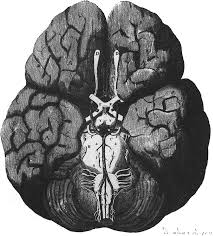
\includegraphics[width=\linewidth]{04_antecedentes/figures/thomas_willis.jpg}
    \end{minipage}
    \hfill
    \begin{minipage}{0.45\linewidth}
        \caption{
            El cerebro de Willis. Del libro \textit{Cerebri Anatome} \citep{willis1664cerebri}. 
            Este grabado representa las arterias cerebrales.
        }
        \label{fig:thomas_willis}
    \end{minipage}
\end{figure}

Esta ciencia ha experimentado transformaciones conceptuales profundas desde sus orígenes. Partiendo del debate entre visiones cardiocéntricas y encefalocéntricas, donde Aristóteles defendía una visión que situaba tanto el alma como las facultades cognitivas en el corazón, y por su parte, Hipócrates y, posteriormente Galeno, argumentaron que el cerebro era la base de la inteligencia y las emociones. Este debate, iniciado en la Grecia clásica encontró su resolución gradual a través de siglos de investigación anatómica y fisiológica \citep{blanco2014historia}.

Este conflicto entre visiones cardiocéntricas y encefalocentristas se mantuvo durante siglos. Galeno de Pérgamo (129-216 d.C.), a través de sus estudios anatómicos en animales, estableció una doctrina que dominaría el pensamiento médico durante más de un milenio: la teoría ventricular. Según esta concepción, los ventrículos cerebrales, las cavidades llenas de líquido en el interior del cerebro, eran los repositorios de las facultades mentales, organizadas jerárquicamente desde la sensación hasta la memoria y el razonamiento \citep{blanco2014historia}.

El siglo XVIII trajo consigo el descubrimiento de la naturaleza eléctrica de la actividad nerviosa, punto que analizaremos y trabajaremos mas adelante, un hallazgo que transformaría para siempre nuestra comprensión del sistema nervioso. Luigi Galvani (1737-1798) demostró en 1791 que la estimulación eléctrica podía provocar contracciones musculares gracias a sus experimentos en ranas, estableciendo que la ``electricidad animal'' era el medio de comunicación nerviosa \citep{blanco2014historia}. Este descubrimiento abrió la puerta a una comprensión del sistema nervioso basada en principios físicos mensurables.

Continuando con el siglo XIX el cual consolidó dos pilares fundamentales de la neurociencia moderna. Por un lado, Santiago Ramón y Cajal estableció la doctrina de la neurona, demostrando que el sistema nervioso está compuesto por células individuales discretas que se comunican a través de contactos especializados, posteriormente denominados sinapsis por Charles Sherrington. Por otro lado, los estudios sobre localización cortical de Paul Broca y Carl Wernicke establecieron que diferentes regiones cerebrales median funciones cognitivas específicas \citep{blanco2014historia}.

El siglo XX presenció avances decisivos para el presente trabajo. Alan Hodgkin y Andrew Huxley desarrollaron en la década de 1950 el primer modelo cuantitativo completo de la excitabilidad neuronal, describiendo los mecanismos iónicos del potencial de acción en el axón gigante del calamar \citep{hodgkin1952quantitative}. Este modelo, que les valió el Premio Nobel de Medicina en 1963, sigue siendo una referencia en la neurociencia computacional y será detallado en la Sección~\ref{subsec:Hodgkin-Huxley}.

\begin{figure}[H]
    \centering
    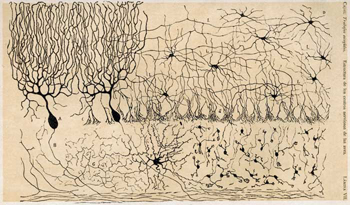
\includegraphics[width=0.55\textwidth]{04_antecedentes/figures/CajalCerebellum.jpg}
    \caption{
        Dibujo de Ramón y Cajal de las células del cerebelo de un pollo, mostrado en ``Estructura de los centros nerviosos de las aves'', Madrid, 1905.
    }
    \label{fig:cajal-cerebelo}
\end{figure}

Complementariamente, los estudios de Henry Dale, Otto Loewi y Bernard Katz establecieron los principios de la transmisión sináptica química, revelando cómo los neurotransmisores median la comunicación entre neuronas \citep{blanco2014historia}. Y finalmente, David Hubel y Torsten Wiesel revolucionaron nuestra comprensión del procesamiento visual cortical en las décadas de 1950 y 1960. Mediante registros electrofisiológicos en la corteza visual de gatos, descubrieron que las neuronas corticales responden selectivamente a características específicas del estímulo, como la orientación de barras luminosas \citep{hubel1959receptive}. Describieron la organización jerárquica del sistema visual, desde células simples que responden a bordes orientados en posiciones específicas, hasta células complejas con mayor invariancia espacial. Su trabajo, reconocido con el Premio Nobel de Medicina en 1981, estableció los principios de selectividad neuronal que fundamentan los modelos computacionales de corteza visual, incluyendo el modelo de \citet{echeveste2020cortical} que implementaremos en este trabajo.

Estos desarrollos históricos convergieron con el nacimiento de las ciencias de la computación para dar lugar a la neurociencia computacional, disciplina que proporciona el marco teórico y metodológico del presente trabajo.

% =============================================================================
% SECCIÓN 2: FUNDAMENTOS BIOLÓGICOS (CITAS CORREGIDAS)
% =============================================================================

\section{Fundamentos biológicos}
\label{sec:fundamentos_biologicos}

Los modelos computacionales de procesamiento neuronal deben fundamentarse en las propiedades biológicas de las neuronas y los circuitos que las interconectan. En esta sección vamos a presentar los principios biológicos esenciales que subyacen a los modelos estudiados en este trabajo, desde los mecanismos iónicos de la señalización neuronal hasta la organización funcional de las áreas corticales involucradas en la percepción visual y multisensorial.

\begin{figure}[H]
    \centering
    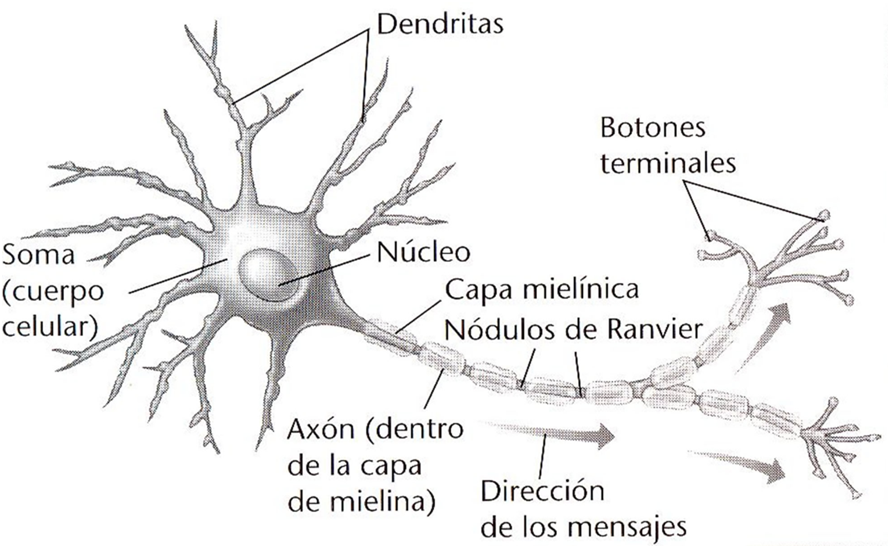
\includegraphics[width=0.65\textwidth]{04_antecedentes/figures/neurona.png}
        \caption{
        Estructura anatómica de una neurona, mostrando sus componentes principales.
    }
    \label{fig:neurona}
\end{figure}

\subsection{La neurona como unidad funcional}
\label{subsec:neurona_unidad}

La neurona es la unidad fundamental de procesamiento del sistema nervioso. Estructuralmente, cada neurona comprende un cuerpo celular o soma que contiene el núcleo y la maquinaria metabólica, dendritas que reciben señales de otras neuronas, un axón que transmite señales hacia células postsinápticas, y terminales sinápticos especializados para la liberación de neurotransmisores \citep{dayan2005theoretical}.

Toda esta estructura está delimitada por una membrana celular cuyas propiedades eléctricas son fundamentales para la comunicación entre neuronas, que depende de cambios rápidos en el potencial eléctrico. En reposo, esta membrana mantiene una diferencia de potencial de aproximadamente $-70$ mV, con el interior de la célula negativo respecto al exterior. Este potencial de reposo se establece mediante canales iónicos selectivos, principalmente permeables a iones de potasio (K$^+$), junto con la acción de bombas iónicas que mantienen los gradientes de concentración \citep{dayan2005theoretical}.

\subsubsection{Canales iónicos y potencial de acción}

Los canales iónicos son proteínas integrales que atraviesan la membrana celular y permiten el paso selectivo de iones específicos. La particularidad de los canales iónicos neuronales es su alta conductancia, del orden de $10^7$ cargas por segundo, lo que permite los cambios rápidos en el potencial de membrana necesarios para generar potenciales de acción \citep{dayan2005theoretical}.

El potencial de acción, descubierto y caracterizado cuantitativamente por \citet{hodgkin1952quantitative}, constituye la señal eléctrica fundamental mediante la cual las neuronas transmiten información a distancia. Su generación depende de dos poblaciones de canales iónicos dependientes de voltaje: los canales de sodio (Na$^+$), cuya apertura produce la despolarización rápida de la membrana, y los canales de potasio (K$^+$), cuya apertura más lenta permite la repolarización. El potencial de acción procede según un patrón de ``todo o nada'', donde todos los impulsos exhiben la misma amplitud, y la intensidad del estímulo se codifica mediante la frecuencia de disparo \citep{dayan2005theoretical}.

El modelo de Hodgkin-Huxley, que será presentado en detalle en la Sección~\ref{subsec:Hodgkin-Huxley}, formaliza matemáticamente estos mecanismos mediante un sistema de ecuaciones diferenciales que describe la dinámica del potencial de membrana en función de las conductancias iónicas dependientes de voltaje.

\begin{figure}[H]
    \centering
    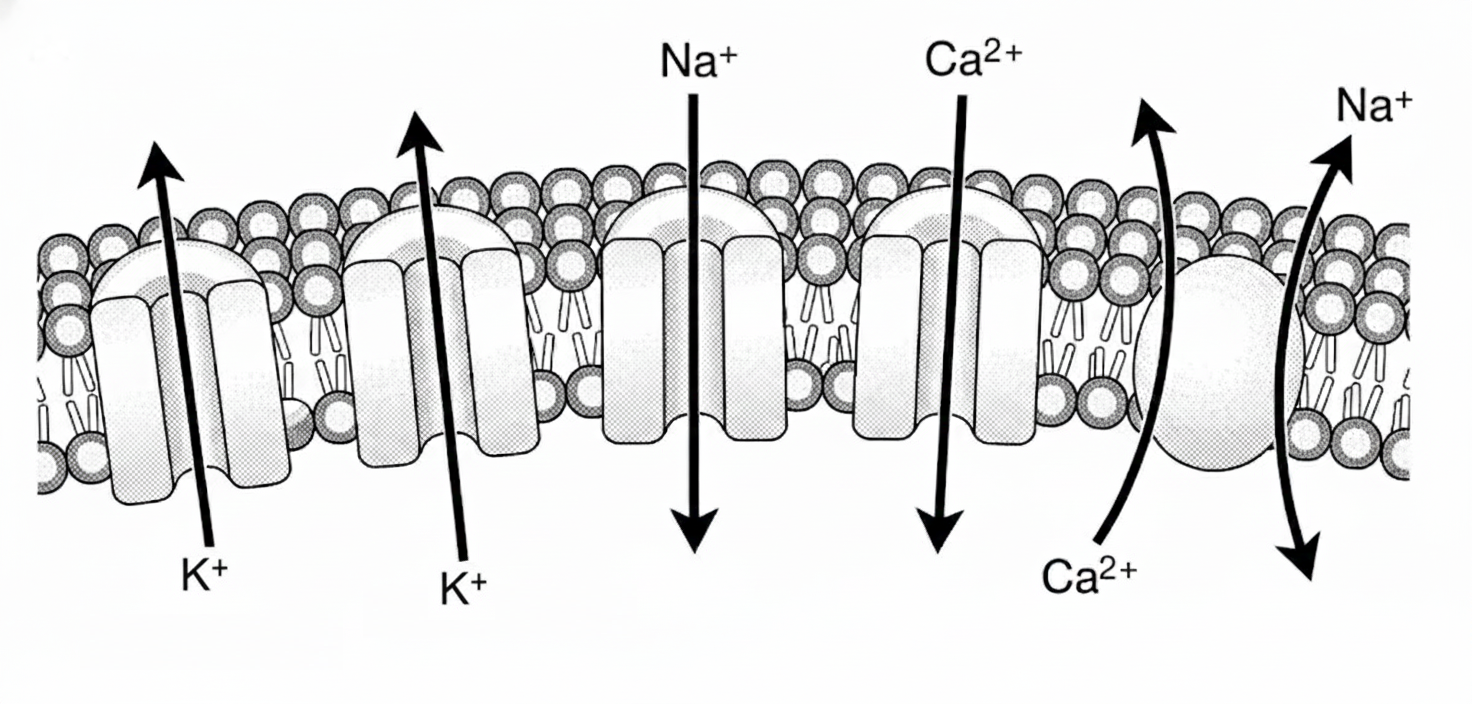
\includegraphics[width=0.75\textwidth]{04_antecedentes/figures/canal-ionico.png}
        \caption{
        Representación esquemática de la membrana neuronal mostrando canales iónicos selectivos.
    }
    \label{fig:canal-ionico}
\end{figure}

\subsubsection{Transmisión sináptica}

La comunicación entre neuronas ocurre predominantemente mediante sinapsis químicas, donde la llegada de un potencial de acción al terminal presináptico desencadena la liberación de neurotransmisores hacia la hendidura sináptica. Estos neurotransmisores se unen a receptores en la membrana de la neurona postsináptica, alterando su conductancia iónica y modificando su potencial eléctrico junto con la probabilidad de que esta genere su propio impulso\citep{dayan2005theoretical}.

Este mecanismo se modela como una transferencia de señales con efectos contrapuestos. Dependiendo del tipo de interacción, la neurona receptora puede sufrir una despolarización (excitación), que aumenta su probabilidad de disparo, o una hiperpolarización (inhibición), que la reduce. Esta distinción funcional permite organizar los modelos de redes neuronales, un tema que explicaremos más adelante en la Sección \ref{subsec:modelos_neuronas}.

\subsection{El sistema visual: de la retina a la corteza}
\label{subsec:sistema_visual}

El sistema visual procesa la información luminosa a través de una serie de estaciones organizadas jerárquicamente: retina, núcleo geniculado lateral del tálamo (LGN), corteza visual primaria (V1), y áreas corticales extraestriadas. En cada nivel aumenta la complejidad de las características extraídas del estímulo visual \citep{dayan2005theoretical}.

\begin{figure}[H]
    \centering
    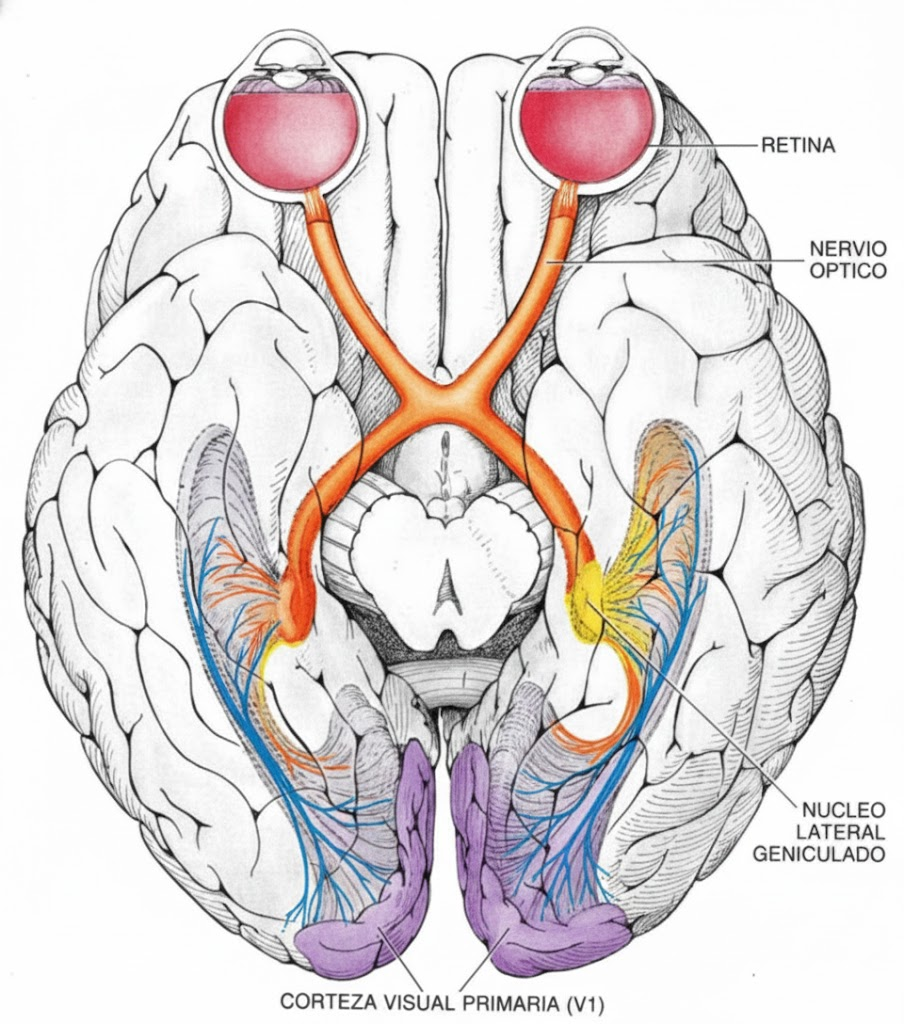
\includegraphics[width=0.65\textwidth]{04_antecedentes/figures/v1.jpg}
        \caption{
        Vía Visual Primaria. Esquema anatómico que muestra el sistema de transmisión de señales visuales.
    }
    \label{fig:patterns/v1}
\end{figure}

\subsubsection{Retina y células ganglionares}

La retina transforma la energía luminosa en señales eléctricas mediante los fotorreceptores: los conos, responsables de la visión en color y de alta resolución en condiciones de buena iluminación, y los bastones, más sensibles pero acromáticos, que permiten la visión en condiciones de baja luminosidad. Esta señal es procesada por circuitos locales antes de llegar a las células ganglionares cuyos axones forman el nervio óptico y constituyen la salida de la retina hacia el cerebro.

Dichas células ganglionares son un tipo de neuronas de axón mielinizado localizadas en la superficie interna de la retina. Se clasifican en dos tipos principales según su tamaño y propiedades funcionales: las células magnocelulares (M), grandes y sensibles al movimiento y contraste, y las células parvocelulares (P), más pequeñas y sensibles al color y detalle fino. Estas neuronas responden a estímulos lumínicos únicamente dentro de una región concreta del espacio visual denominada campo receptivo, y sus respuestas dependen del contraste entre regiones iluminadas y oscuras \citep{dayan2005theoretical}. Los campos receptivos de las células ganglionares presentan una organización centro-periferia antagonista: las células centro-ON se excitan con luz en el centro de su campo receptivo y se inhiben con luz en la periferia, mientras que las células centro-OFF presentan el patrón inverso. Esta distinción nos sera útil en los siguientes párrafos.

\subsubsection{Núcleo geniculado lateral}

El \acrfull{LGN}, localizado en el tálamo dorsal, constituye la principal estación de procesamiento y relevo entre la retina y la corteza visual primaria (V1). Actúa como un sofisticado filtro que organiza y modula el flujo de información en el marco de un procesamiento jerárquico.

Estructuralmente, el \acrshort{LGN} preserva de forma estricta la organización retinotópica y mantiene la segregación de las vías funcionales paralelas que emergen de la retina a través de una organización laminar especializada (capas físicas). Las capas magnocelulares (capas 1-2) reciben aferencias de las células ganglionares M, especializándose en la detección de movimiento y bajas frecuencias espaciales con una alta velocidad de conducción. Por su parte, las capas parvocelulares (capas 3-6) reciben información de las células P, procesando detalles finos y color (ejes rojo-verde). Entre estas capas se sitúan las zonas koniocelulares, que reciben información de las células K, vinculadas al procesamiento del espectro azul-amarillo \citep{dayan2005theoretical}.

Funcionalmente, las neuronas del \acrshort{LGN} presentan campos receptivos con una organización centro-periferia antagonista (células ON y OFF), similar a las células ganglionares de la retina. Sin embargo, la importancia de esta etapa reside en cómo dicha configuración facilita las transformaciones de orden superior en la jerarquía visual. La convergencia espacial de múltiples neuronas del \acrshort{LGN}, cuyos campos receptivos se alinean en el espacio visual, permite que las neuronas en la capa 4 de V1 desarrollen selectividad a la orientación de bordes, una característica inexistente en etapas previas.

Un aspecto crítico de su fisiología es la asimetría en sus conexiones: aunque el flujo principal de información visual es feedforward (Retina $\rightarrow$ LGN $\rightarrow$ V1), el \acrshort{LGN} recibe una cantidad significativamente mayor de conexiones feedback desde la corteza visual. Mientras que las señales de la retina actúan como ``conductores'' (\textit{drivers}) de la respuesta sensorial, las conexiones corticales feedback funcionan como ``moduladores''. Este sistema de retroalimentación permite que niveles jerárquicos superiores (V1) regulen la ganancia de contraste y ejecuten mecanismos de atención selectiva, filtrando activamente la información que debe ser transmitida a la corteza según las demandas de la tarea visual \citep{dayan2005theoretical}. Así, el \acrshort{LGN} se establece como la primera compuerta talamocortical donde el contexto y la predicción comienzan a dar forma a la percepción sensorial.

\subsubsection{Corteza visual primaria (V1)}

La corteza visual primaria, también conocida como área V1 o corteza estriada, constituye la primera estación de procesamiento cortical de la información visual. Como toda la corteza cerebral, V1 se organiza en seis capas horizontales numeradas del 1 al 6 desde la superficie hacia el interior. Cada capa tiene una composición celular y patrones de conectividad característicos: la capa 4 recibe las entradas principales desde el LGN, mientras que otras capas procesan esta información y la transmiten a otras regiones corticales.

\citet{hubel1959receptive} descubrieron que las neuronas de V1 responden selectivamente a características específicas de los estímulos, particularmente a bordes y barras con orientaciones determinadas, una propiedad ausente en las células ganglionares y del \acrshort{LGN}. A su vez, identificaron dos tipos principales de neuronas en V1. Las \textit{células simples}, ubicadas principalmente en la capa 4, presentan campos receptivos con regiones ON y OFF separadas espacialmente, respondiendo a bordes orientados en posiciones específicas del campo visual. Cada célula simple está afinada para detectar estímulos con orientaciones en un rango de aproximadamente diez grados \citep{blanco2014historia}. Y las \textit{células complejas}, localizadas en las capas 2, 3, 5 y 6, responden también a bordes orientados pero con mayor invariancia a la posición exacta del estímulo dentro de su campo receptivo, que es más amplio que el de las células simples. El modelo de Hubel y Wiesel propone que la selectividad a orientación de las células simples surge de la convergencia de entradas desde células del LGN con campos receptivos alineados \citep{dayan2005theoretical}.

En V1, las neuronas con propiedades de respuesta similares se organizan en columnas verticales que atraviesan las diferentes capas corticales. Las columnas de orientación, de entre 30 y 100 micrómetros de grosor, agrupan neuronas que responden a la misma orientación preferida. Estas columnas se disponen sistemáticamente de modo que un recorrido tangencial a través de la corteza encuentra secuencialmente todas las orientaciones posibles. Las columnas de dominancia ocular alternan el predominio de respuesta al ojo izquierdo y derecho. El conjunto de columnas que representa un ciclo completo de orientaciones para ambos ojos, junto con las estructuras denominadas ``blobs'' que procesan información de color, constituye una \textit{hipercolumna} de aproximadamente un milímetro cuadrado \citep{blanco2014historia, dayan2005theoretical}. Esta organización modular se repite a lo largo de toda la superficie de V1.

Esta arquitectura columnar es directamente relevante para el modelo de Echeveste, que simula precisamente una hipercolumna de V1 como unidad funcional para la inferencia probabilística sobre orientaciones visuales, como se detallará en el Capítulo~\ref{chapter:modelos_estudiados}.

\begin{figure}[H]
    \centering
    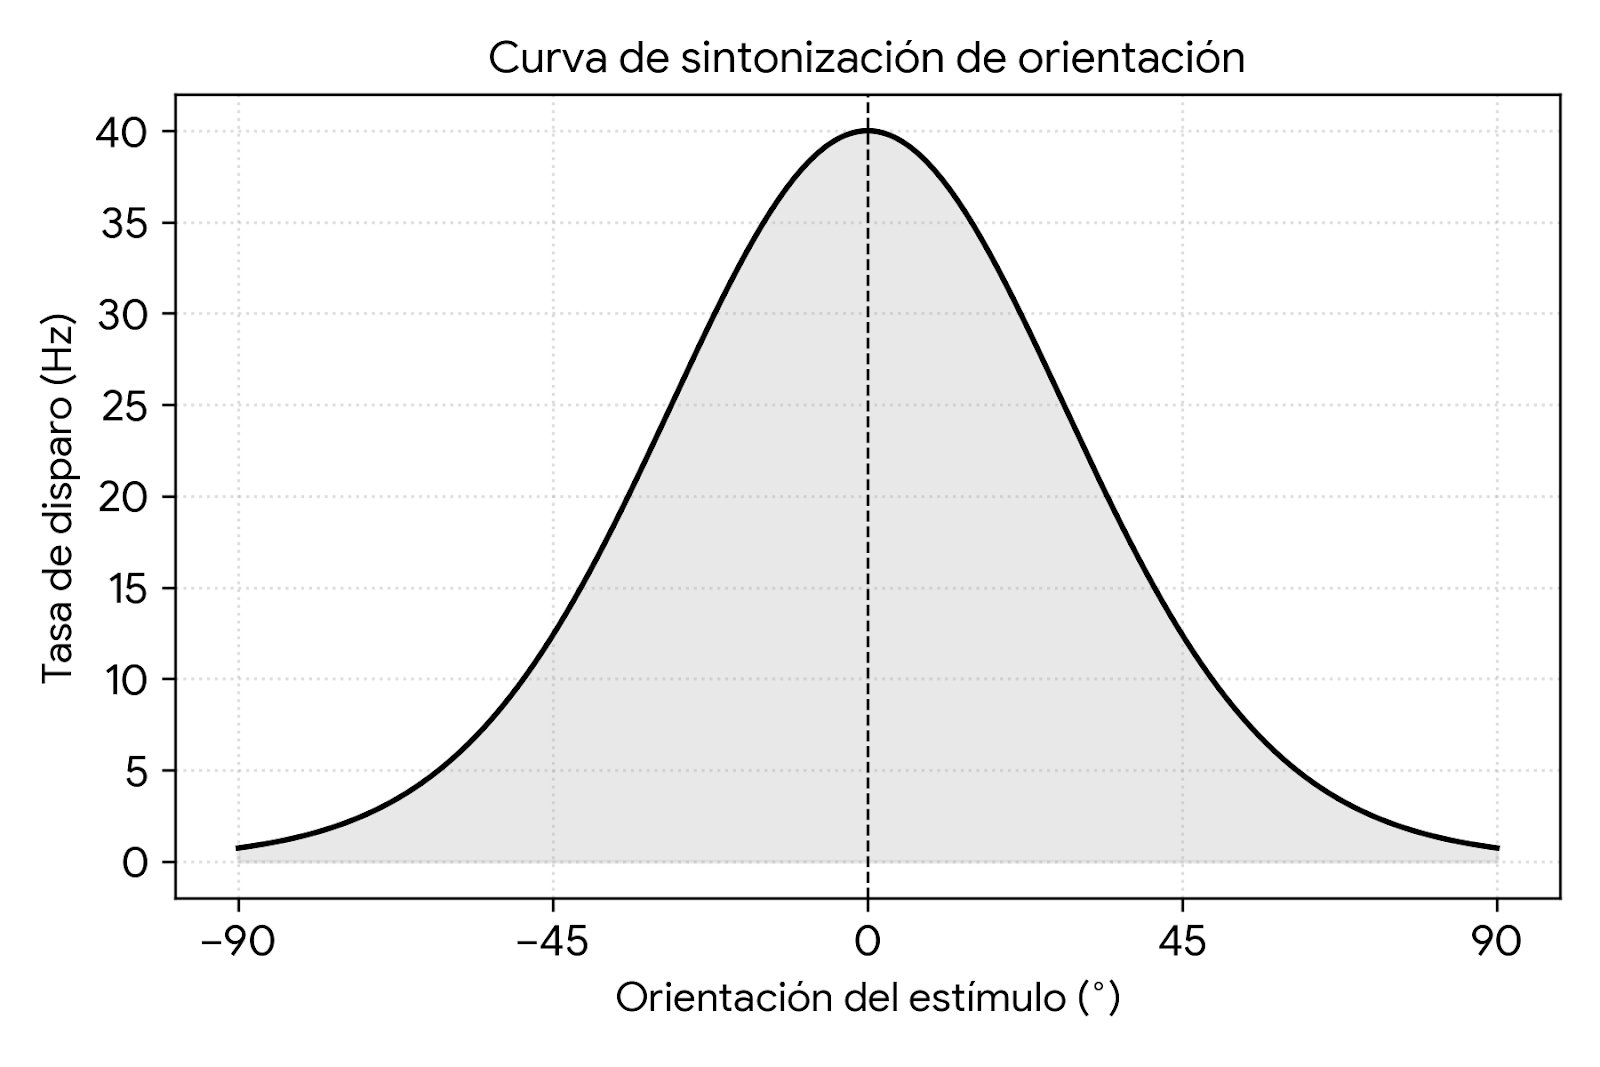
\includegraphics[width=0.85\textwidth]{04_antecedentes/figures/tuning-curbe.png}
    \caption{
    Curva de sintonización (tuning curve) de orientación de una neurona en V1. La respuesta (tasa de disparo en Hz) es máxima ante una orientación específica del estímulo y decrece conforme la inclinación del borde se desvía de la preferencia de la neurona.
    }
    \label{fig:tuning-curbe}
\end{figure}

\subsection{Filtros de Gabor como modelo de campos receptivos}
\label{subsec:filtros_gabor}

Los campos receptivos de las células simples de V1, con sus regiones ON y OFF, pueden aproximarse matemáticamente. Una función de Gabor es el producto de una función gaussiana, que define la extensión espacial del campo receptivo, y una función sinusoidal, que captura la estructura de bandas claras y oscuras \citep{dayan2005theoretical}:

\begin{equation}
D_s(x, y) = \frac{1}{2\pi\sigma_x\sigma_y} \exp\left(-\frac{x^2}{2\sigma_x^2} - \frac{y^2}{2\sigma_y^2}\right) \cos(kx - \phi)
\label{eq:gabor_function}
\end{equation}

Los parámetros de esta función determinan las propiedades del campo receptivo: $\sigma_x$ y $\sigma_y$ controlan la extensión espacial en las direcciones horizontal y vertical respectivamente, $k$ es la frecuencia espacial preferida que determina el espaciado entre bandas claras y oscuras, y $\phi$ es la fase espacial preferida que determina dónde caen los límites entre regiones ON y OFF dentro del campo receptivo. Estudios experimentales han demostrado que las funciones de Gabor proporcionan excelentes aproximaciones a los campos receptivos medidos en células simples de la corteza visual de gatos y primates \citep{dayan2005theoretical}.

La orientación preferida de un filtro de Gabor se obtiene rotando el sistema de coordenadas. Y finalmente una neurona con orientación preferida $\theta$, responde máximamente a bordes orientados en dicha dirección. Estos filtros juegan un papel central en el \acrfull{GSM} utilizado por \citet{echeveste2020cortical} el cual se explicará en el Capítulo \ref{chapter:modelos_estudiados}. 

\begin{figure}[H]
    \centering
    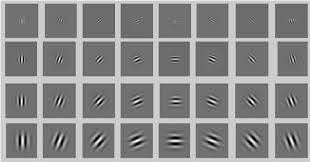
\includegraphics[width=0.75\textwidth]{04_antecedentes/figures/gabor-bank.jpg}
    \caption{
    Banco de filtros de Gabor utilizados para modelar los campos receptivos de las células simples en V1. Cada subfigura representa un filtro con una combinación específica de orientación ($\theta$) y frecuencia espacial ($k$). La extensión espacial de cada campo receptivo está dada por $\sigma_x$ y $\sigma_y$ en la Ecuación~\ref{eq:gabor_function}.
    }
    \label{fig:gabor-banks}
\end{figure}

\subsection{Vías visuales: procesamiento paralelo}
\label{subsec:vias_visuales}

Después del procesamiento inicial en V1, la información visual se distribuye a través de múltiples áreas corticales extraestriadas organizadas en dos corrientes principales de procesamiento paralelo \citep{dayan2005theoretical}:

\textbf{La vía ventral} se proyecta desde V1 hacia V2, V4 y la corteza inferotemporal. Esta vía se especializa en el reconocimiento de objetos, procesando información sobre forma, color e identidad. Lesiones en esta vía producen agnosias visuales, dificultades para reconocer objetos a pesar de una visión básica preservada.

\textbf{La vía dorsal} se proyecta desde V1 hacia V2, el área MT (V5) y la corteza parietal posterior. Esta vía procesa información sobre movimiento, localización espacial y guía de acciones motoras. Lesiones en esta vía producen déficits en la localización de objetos y en la coordinación visomotora.

Esta división funcional tiene implicaciones directas para los modelos que estudiaremos. El modelo de Echeveste, que representa características visuales como la orientación en una hipercolumna de V1, está más relacionado con el procesamiento de la vía ventral. En contraste, el modelo de Cuppini, que representa la localización espacial de estímulos audiovisuales, está más relacionado con el procesamiento de la vía dorsal. Como se discutirá en el Capítulo~\ref{chapter:modelos_estudiados}, la eventual integración de ambos enfoques requerirá considerar cómo interactúan estos diferentes tipos de representaciones corticales.

\subsection{El colículo superior y la integración multisensorial}
\label{subsec:coliculo_superior}

El \acrfull{CS} es una estructura del mesencéfalo que desempeña un papel fundamental en la orientación de la atención y los movimientos oculares hacia estímulos relevantes del entorno. A diferencia de las áreas corticales discutidas anteriormente, el \acrshort{CS} recibe información de múltiples modalidades sensoriales, visual, auditiva y somatosensorial, organizándolas en mapas topográficos superpuestos \citep{stein2012new}.

El \acrshort{CS} se organiza en capas funcionalmente diferenciadas: las capas superficiales procesan predominantemente información visual y mantienen una representación retinotópica del campo visual, mientras que las capas profundas son multimodales y contienen neuronas que responden a estímulos de diferentes modalidades cuando estos provienen de ubicaciones espaciales coincidentes. Esta convergencia anatómica de información multisensorial hace del \acrshort{CS} un punto ideal para estudiar los mecanismos de integración sensorial.

Estudios electrofisiológicos en el \acrshort{CS} han revelado principios fundamentales de la integración multisensorial que los modelos computacionales deben capturar \citep{stein2012new, paredes2025scikit}. La \textit{regla espacial} establece que estímulos de diferentes modalidades cercanos en el espacio producen respuestas potenciadas (superaditivas) comparadas con las respuestas unimodales, mientras que estímulos distantes producen respuestas deprimidas. La \textit{regla temporal} indica que la integración es máxima cuando los estímulos de diferentes modalidades son cercanos en el tiempo. Y la \textit{regla de efectividad inversa} establece que la potenciación multisensorial es mayor cuando los estímulos unimodales individuales son débiles o ambiguos \citep{cuppini2017biologically}.

El modelo de Cuppini, que será presentado en el Capítulo~\ref{chapter:modelos_estudiados}, captura estos principios mediante una arquitectura de tres capas donde las regiones unisensoriales están organizadas topográficamente y conectadas a una capa de inferencia causal que determina si estímulos audiovisuales provienen de una fuente común o de fuentes independientes.

\subsection{De la biología a la computación}
\label{subsec:sintesis_biologia}

Los fundamentos biológicos presentados en esta sección establecen las restricciones y fenómenos que los modelos computacionales de procesamiento neuronal deben capturar. La organización jerárquica del sistema visual, desde los campos receptivos en la retina hasta la selectividad a orientación en V1, proporciona el sustrato para el modelo de Echeveste. A su vez, la integración multisensorial en estructuras como el colículo superior, con sus principios de coincidencia espacial y temporal, fundamenta el modelo de Cuppini.

Ya desarrolladas las restricciones biológicas fundamentales. La siguiente sección presenta el marco formal de la neurociencia computacional que permite formalizar estas restricciones y evaluar las capacidades de los modelos resultantes.

% =============================================================================
% SECCIÓN 2: NEUROCIENCIA COMPUTACIONAL
% =============================================================================

\section{Neurociencia computacional}
\label{sec:neuro_computacional}

La neurociencia computacional representa una síntesis moderna de neurobiología, matemáticas y ciencias de la computación, orientada a comprender cómo el sistema nervioso procesa información y genera comportamiento. Esta disciplina no se limita a simular fenómenos neuronales, también busca identificar los principios computacionales fundamentales que subyacen a las funciones cerebrales y estudiar como estos métodos matemáticos, físicos e informáticos pueden proporcionar información importante sobre el funcionamiento del sistema nervioso \citep{dayan2005theoretical}.

\subsection{Los tres niveles}
\label{subsec:marr_niveles}

Un marco conceptual fundamental para la neurociencia computacional fue propuesto por \citet{marr2010vision} en su influyente obra \textit{Vision}. Donde argumentó que cualquier sistema de procesamiento de información puede ser analizado en tres niveles distintos, pero complementarios \citep{marr2010vision}:

El \textbf{nivel computacional} aborda la pregunta de \textit{qué} computa el sistema y \textit{por qué}. En este nivel, se especifica el problema computacional que el sistema debe resolver y la lógica de la estrategia mediante la cual puede resolverse. Por ejemplo, para la corteza visual, el problema computacional podría ser inferir las características más probables de un estímulo (como su orientación o contraste) a partir de información sensorial ruidosa, representando no solo una estimación puntual, sino la incertidumbre asociada a dicha estimación.

El \textbf{nivel algorítmico} pregunta \textit{cómo} se lleva a cabo ese cómputo, sin comprometerse todavía con el sustrato físico que lo ejecuta. ¿Qué representaciones utiliza el sistema? ¿Qué algoritmos transforman estas representaciones? Este nivel especifica los procedimientos concretos mediante los cuales se resuelve el problema computacional.

Finalmente, el \textbf{nivel de implementación} se ocupa de cómo los circuitos neuronales implementan el algoritmo. ¿Qué circuitos neuronales realizan el cómputo? ¿Cómo se codifica la información en patrones de actividad neuronal? Por ejemplo, en el caso de la inferencia probabilística, esto implica especificar cómo redes recurrentes de neuronas, pueden implementar el muestreo de distribuciones posteriores.

Esta jerarquía de niveles proporciona una estructura para organizar nuestro conocimiento del cerebro y, específicamente, para conectar descripciones funcionales con mecanismos neuronales. En este trabajo, donde buscamos implementar un modelo de inferencia causal multisensorial con dinámicas corticales realistas, se opera precisamente en la interfaz entre estos niveles: partimos de una especificación computacional (inferencia bayesiana) y buscamos su implementación en circuitos neuronales biológicamente plausibles.

\subsection{Codificación y decodificación neuronal}
\label{subsec:codificacion_neuronal}

Una cuestión central en neurociencia computacional es cómo las neuronas representan información sobre el mundo externo y los estados internos del organismo. La investigación en este ámbito se ha centrado en dos problemas complementarios: la \textit{codificación neuronal} (cómo los estímulos se traducen en patrones de actividad neuronal) y la \textit{decodificación neuronal} (cómo la información puede extraerse de estos patrones) \citep{dayan2005theoretical}.

El patrón neuronal más estudiado tradicionalmente es la \textbf{tasa de disparo}: la frecuencia promedio de potenciales de acción generados por una neurona en un intervalo de tiempo dado. Estudios clásicos de Adrian en la década de 1920 demostraron que la intensidad de un estímulo se correlaciona con la tasa de disparo de las neuronas sensoriales \citep{blanco2014historia}. Sin embargo, trabajos recientes han propuesto que el \textbf{potencial de membrana} en sí mismo puede servir como variable representacional. En este enfoque, no solo el valor medio del potencial sino también su variabilidad codifica información relevante sobre el estímulo y la incertidumbre asociada a su estimación. La tasa de disparo se deriva entonces como una transformación no lineal del potencial de membrana.

Esta relación entre potencial de membrana y tasa de disparo tiene implicaciones importantes para la codificación poblacional. Cuando múltiples neuronas representan conjuntamente un estímulo, la distribución de sus potenciales de membrana puede codificar no solo una estimación puntual de las características del estímulo, sino toda una distribución de probabilidad que refleja la incertidumbre perceptual. Por todo esto, la elección de cómo modelar la dinámica neuronal determina qué tipo de información puede ser codificada y posteriormente decodificada del patrón de actividad poblacional. En la Sección~\ref{sec:modelo_echeveste} exploraremos en detalle cómo esta idea se formaliza matemáticamente en el contexto de la inferencia probabilística.

\subsection{Modelos de neuronas}
\label{subsec:modelos_neuronas}

La neurociencia computacional ha desarrollado una variedad de modelos de neuronas con diferentes niveles de detalle biofísico, desde descripciones detalladas que involucran miles de ecuaciones diferenciales acopladas hasta simplificaciones útiles para estudiar grandes redes interconectadas. La elección del modelo apropiado depende de las preguntas que se desean abordar y del compromiso entre realismo biológico y tratabilidad computacional \citep{dayan2005theoretical}.

\subsubsection{El modelo de Hodgkin-Huxley}
\label{subsec:Hodgkin-Huxley}

El modelo Hodgkin-Huxley constituye una de las bases del modelado biofísico de neuronas \citep{hodgkin1952quantitative}. Desarrollado a partir de experimentos en el axón gigante del calamar, este modelo describe cómo los potenciales de acción surgen de la apertura y cierre de canales iónicos dependientes de voltaje. El modelo integra propiedades eléctricas fundamentales de la membrana neuronal: la capacitancia de membrana $C_m$, las conductancias de los canales de sodio, potasio y fuga ($\bar{g}_{Na}$, $\bar{g}_K$ y $g_L$), y la actividad de las puertas iónicas descrita por las variables $m$, $h$ y $n$, que se abren y cierran con tasas dependientes del voltaje. Estas propiedades se relacionan mediante un sistema de cuatro ecuaciones diferenciales acopladas, cuya ecuación principal describe la dinámica del potencial de membrana $V$:
\begin{equation}
C_m \frac{dV}{dt} = -\bar{g}_{Na}m^3h(V-E_{Na}) - \bar{g}_K n^4(V-E_K) - g_{L}(V-E_{L}) + I_{ext}
\label{eq:hodgkin_huxley}
\end{equation}
El modelo captura cuantitativamente la generación del potencial de acción, incluyendo su forma característica y el período refractario \citep{dayan2005theoretical}. Sin embargo, su complejidad computacional lo hace impráctico para simulaciones de redes grandes.

\subsubsection{El modelo integra-y-dispara}

Para simulaciones a mayor escala, se emplean modelos simplificados que capturan las características esenciales de la dinámica neuronal. El modelo integra y dispara (\ac{LIF}) es quizás el más ampliamente utilizado. Según \cite{eliasmith2003neural}, este modelo representa un balance conveniente entre realismo neuronal y tratabilidad computacional ya que introduce la no linealidad más prominente de los sistemas neuronales, el potencial de acción, mientras mantiene una formulación matemática simple:

\begin{equation}
\tau_m \frac{dV}{dt} = -(V - V_{rest}) + R_m I(t)
\label{eq:lif}
\end{equation}
donde $V$ es el potencial de membrana, $\tau_m$ es la constante de tiempo de membrana, $V_{rest}$ es el potencial de reposo, $R_m$ es la resistencia de membrana, e $I(t)$ es la corriente de entrada. Cuando $V$ alcanza un umbral $V_{th}$, se registra un potencial de acción y el potencial se reinicia a un valor $V_{reset}$.

A pesar de su simplicidad, el modelo LIF reproduce muchas propiedades cualitativas de neuronas reales, incluyendo la variabilidad en los tiempos de disparo y la sensibilidad a fluctuaciones en la entrada \citep{dayan2005theoretical}.

\begin{figure}[H]
    \centering
    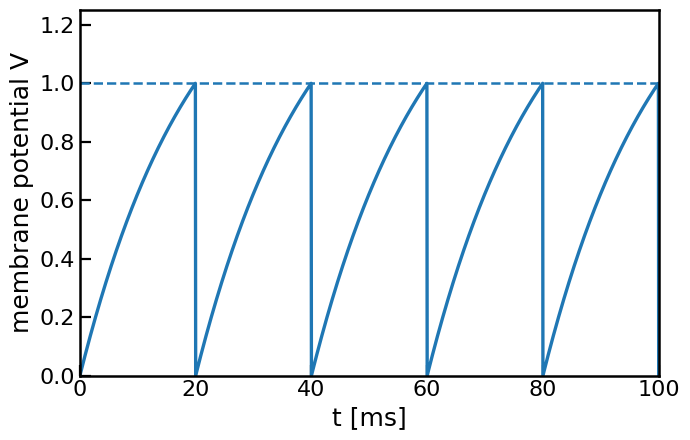
\includegraphics[width=0.55\textwidth]{04_antecedentes/figures/integrate_fire.png}
    \caption{
        Evolución temporal del potencial de membrana $V$ de una neurona \textit{integra-y-dispara} impulsada por una corriente constante. Para mayor claridad, el potencial se presenta normalizado respecto al umbral de disparo ($V_{th} = 1.0$) y el reposo ($V_{reset} = 0$).
    }
    \label{fig:integrate_fire}
\end{figure}

\subsubsection{Modelos de tasa}

En un nivel aún más abstracto, los \textbf{modelos de tasa} (\textit{rate models}) describen la actividad neuronal en términos de la tasa de disparo promedio de poblaciones de neuronas, ignorando los tiempos precisos de los potenciales de acción individuales \citep{dayan2005theoretical}. Una formulación común es:

\begin{equation}
\tau \frac{dr}{dt} = -r + f\left(\sum_j w_{ij} r_j + h_i\right)
\label{eq:rate_model}
\end{equation}

donde $r$ es la tasa de disparo, $f(\cdot)$ es una función de transferencia no lineal (típicamente sigmoide o rectificadora), $w_{ij}$ son los pesos sinápticos, y $h_i$ es la entrada externa.

Los modelos de tasa son computacionalmente eficientes y han sido ampliamente utilizados para estudiar fenómenos como la memoria de trabajo, la toma de decisiones, y la integración sensorial. Sin embargo, al promediar la actividad neuronal, no capturan la variabilidad temporal que caracteriza la actividad cortical real \citep{gerstner2002spiking}.

\subsubsection{Neuronas estocásticas con dinámica de membrana}

El modelo neuronal propuesto por \cite{echeveste2020cortical}, el cual es el objeto de estudio de este trabajo, ocupa un lugar intermedio en la jerarquía de complejidad presentada. A diferencia de los modelos de tasa puros, este enfoque mantiene el potencial de membrana como variable dinámica principal, permitiendo que su variabilidad temporal codifique información. A diferencia del modelo LIF, no implementa un mecanismo de disparo explícito con umbral y reinicio, sino que deriva la tasa de disparo como una transformación continua y supralineal del potencial de membrana.

Crucialmente, este tipo de modelo incorpora dos características biológicas fundamentales: ruido estocástico que genera variabilidad en las respuestas, y la distinción explícita entre poblaciones excitatorias e inhibitorias, respetando el principio de Dale (cada neurona libera el mismo tipo de neurotransmisor en todas sus sinapsis, siendo exclusivamente excitatoria o inhibitoria). Estas características resultan esenciales para implementar inferencia probabilística mediante muestreo, como se desarrollará en profundidad en la Sección~\ref{sec:modelo_echeveste}.

En síntesis, los modelos presentados representan diferentes compromisos entre fidelidad biofísica y tratabilidad computacional. Sin embargo, las propiedades computacionales de estos modelos dependen no solo de la dinámica de neuronas individuales, sino fundamentalmente de cómo estas se conectan formando redes. En la siguiente sección exploraremos cómo la arquitectura de conexiones recurrentes entre poblaciones excitatorias e inhibitorias da lugar a dinámicas corticales complejas.

\subsection{Conexiones neuronales}
\label{subsec:conexiones_neuronales}

Los modelos de neuronas individuales descritos anteriormente constituyen los bloques fundamentales del procesamiento neuronal. Sin embargo, las funciones cognitivas emergen de la interacción coordinada de miles o millones de neuronas conectadas en redes. La arquitectura de red, forma en que estas neuronas se conectan, determina en gran medida las capacidades computacionales del circuito. Según \cite{dayan2005theoretical}, existen tres clases principales de interconexiones en los circuitos neuronales.

Las \textbf{conexiones feedforward} traen información desde una región ubicada en una etapa anterior de procesamiento hacia una etapa posterior. Computacionalmente, las redes feedforward llamadas así por implementar solo este tipo de conexiones, implementan transformaciones jerárquicas donde cada capa extrae características progresivamente más abstractas de la entrada. Esta arquitectura es eficiente para tareas de clasificación y reconocimiento de patrones, y ha inspirado modelos exitosos como las redes convolucionales en aprendizaje profundo \citep{heaton2018ian}. Sin embargo, las redes puramente feedforward tienen limitaciones importantes: no pueden mantener información en ausencia de entrada, ni generar dinámicas temporales complejas.

\begin{figure}[H]
    \centering
    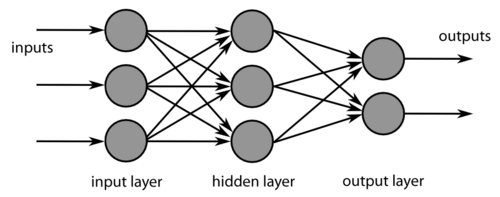
\includegraphics[width=0.55\textwidth]{04_antecedentes/figures/feed-forward.png}
    \caption{
        Modelo computacional de red neuronal feed-forward de una sola capa oculta.
    }
    \label{fig:feed-forward}
\end{figure}

Las \textbf{conexiones feedback} llevan señales de regreso desde etapas posteriores del procesamiento hacia etapas anteriores. El número de fibras feedforward y feedback entre regiones conectadas es típicamente comparable \citep{dayan2005theoretical}. Computacionalmente, estas conexiones permiten que información contextual y expectativas de niveles superiores modulen el procesamiento en niveles inferiores, implementando mecanismos como atención selectiva y codificación predictiva.

\begin{figure}[H]
    \centering
    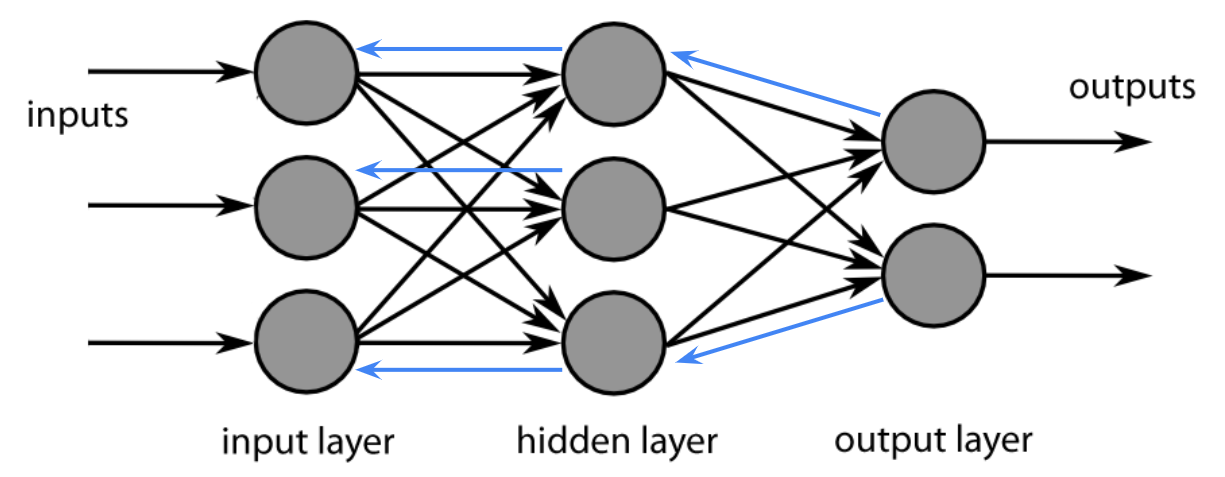
\includegraphics[width=0.55\textwidth]{04_antecedentes/figures/top-down.png}
    \caption{
    Arquitectura de red neuronal con conexiones feedforward e incluyendo conexiones feedback resaltadas en azul.
    }
    \label{fig:top-down}
\end{figure}

Las \textbf{conexiones recurrentes} interconectan neuronas dentro de una misma etapa de procesamiento. Una observación fundamental es que las sinapsis recurrentes típicamente superan en número a las conexiones feedforward o feedback \citep{dayan2005theoretical}. Esta preponderancia tiene profundas implicaciones computacionales: mientras que las redes feedforward transforman la información de manera estática, las redes con conectividad recurrente pueden generar dinámicas temporales complejas. Entre las capacidades únicas de las redes recurrentes se encuentran: \textbf{actividad sostenida} en ausencia de entrada externa, \textbf{amplificación selectiva} de señales débiles, \textbf{fenómenos oscilatorios} en diversas bandas de frecuencia, y formación de \textbf{estados atractores} que pueden servir como memorias asociativas \citep{dayan2005theoretical}.

Dada la importancia de la conectividad recurrente para las funciones computacionales que nos interesan en este trabajo, en la siguiente sección exploraremos en detalle las propiedades de las redes recurrentes y las dinámicas que emergen de ellas.

\begin{figure}[H]
    \centering
    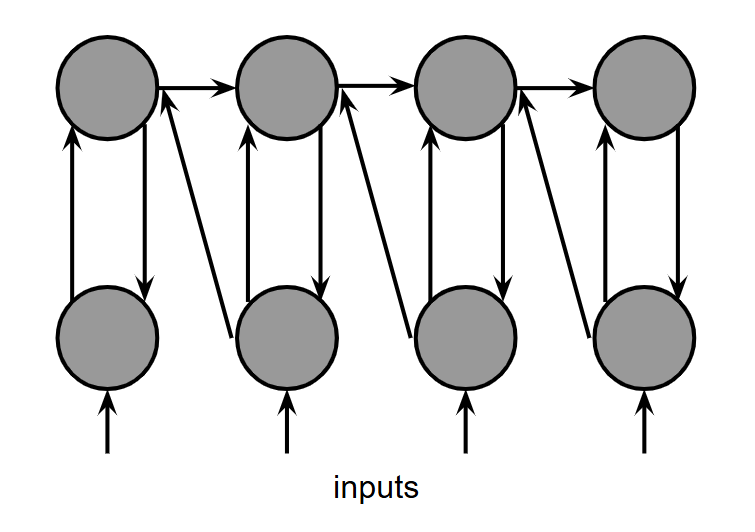
\includegraphics[width=0.5\textwidth]{04_antecedentes/figures/red-recurrente.png}
    \caption{
    Arquitectura de red recurrente. Las conexiones horizontales entre neuronas de la misma capa y las conexiones bidireccionales entre capas permiten que la actividad de cada neurona influya sobre sus vecinas, generando dinámicas temporales complejas.
    }
    \label{fig:red-recurrente}
\end{figure}

\subsection{Redes neuronales recurrentes y dinámicas corticales}
\label{subsec:redes_recurrentes}

Los circuitos corticales se caracterizan por conexiones recurrentes abundantes que pueden clasificarse según su efecto sobre la neurona postsináptica: las \textbf{conexiones excitatorias} aumentan el potencial de membrana, incrementando la probabilidad de disparo, mientras que las \textbf{conexiones inhibitorias} lo disminuyen, reduciendo dicha probabilidad. En el contexto del modelado computacional, esta distinción suele formalizarse mediante el \textbf{principio de Dale}, que asume que cada neurona libera el mismo tipo de neurotransmisor en todas sus sinapsis, clasificándose como excitatoria o inhibitoria. Si bien la evidencia actual muestra que las neuronas biológicas pueden co-liberar múltiples neurotransmisores, esta simplificación resulta útil para construir modelos tratables computacionalmente \citep{dale1935pharmacology}.

La interacción entre poblaciones excitatorias e inhibitorias da lugar a dinámicas complejas que van más allá de la simple transmisión de información feedforward \citep{dayan2005theoretical}. Como se mencionó anteriormente, si las conexiones recurrentes son suficientemente fuertes, el patrón de actividad poblacional puede volverse parcialmente independiente de la estructura de la entrada, permitiendo que la red mantenga estados de actividad que proveen memoria de entradas previas.

Un fenómeno particularmente importante que emerge de las redes recurrentes son las \textbf{oscilaciones neuronales}. Las interacciones entre poblaciones excitatorias e inhibitorias pueden generar actividad oscilatoria en diversas bandas de frecuencia, incluyendo oscilaciones gamma (30-80 Hz) que han sido asociadas con el procesamiento sensorial y la atención \citep{echeveste2020cortical}. Estas oscilaciones no son simples fenómenos sino que pueden cumplir roles funcionales específicos en el procesamiento de información.

Un modelo particularmente influyente que captura estas propiedades es la \textbf{red supralineal estabilizada} (\acrshort{SSN}, \textit{Stabilized Supralinear Network}), que incorpora propiedades esenciales de los circuitos corticales. Este modelo incluye poblaciones separadas de neuronas excitatorias e inhibitorias, funciones de transferencia supralineales (expansivas) consistentes con observaciones experimentales en neuronas corticales, y conectividad recurrente que estabiliza la actividad del circuito \citep{echeveste2020cortical}.

El SSN reproduce fenómenos corticales importantes como la normalización divisiva (un cómputo canónico de circuitos corticales), las respuestas transitorias al inicio de estímulos, y las oscilaciones gamma cuya frecuencia aumenta con el contraste del estímulo. Crucialmente, este modelo constituye la base arquitectónica del trabajo de \cite{echeveste2020cortical}, quienes demostraron cómo extenderlo para implementar inferencia probabilística basada en muestreo. Los detalles matemáticos completos de esta extensión, incluyendo la dinámica neuronal, la función de transferencia supralineal, el rol del ruido estocástico, y cómo estas propiedades emergen del objetivo de muestreo, se presentan en la Sección~\ref{sec:modelo_echeveste}.

% =============================================================================
% SECCIÓN 3: INTEGRACIÓN MULTISENSORIAL
% =============================================================================

\section{Integración multisensorial}
\label{sec:integracion_multisensorial}

La percepción de los estímulos que nos rodean rara vez depende de una única modalidad sensorial. Cuando conversamos con alguien, integramos información visual de los movimientos de sus labios con las señales auditivas de su voz. Esta integración de información proveniente de múltiples sentidos, conocida como \textbf{integración multisensorial}, es un proceso neuronal fundamental que mejora nuestra capacidad para percibir y actuar en el mundo \citep{stein2012new}.

\subsection{La percepción como inferencia probabilística}
\label{subsec:percepcion_bayesiana}

La inferencia probabilística proporciona una solución al problema de formar percepciones al mezclar información parcial y ruidosa de múltiples fuentes, incluyendo diferentes señales sensoriales, modalidades y formas de memoria \citep{echeveste2020cortical}. Formalmente, esta fusión resulta en una \textbf{distribución posterior} que expresa la probabilidad de que características relevantes del entorno sean interpretadas de diferentes formas, dada la información disponible a través de los sentidos.

Dado que, por ejemplo, el sistema visual solo tiene acceso a los fotones absorbidos en la retina, la interpretación de los objetos requiere ir más allá de la información directamente disponible. El cerebro debe entonces \textit{inferir} las propiedades del mundo externo a partir de esta información sensorial comúnmente incompleta y ruidosa. El teorema de Bayes nos proporciona el marco formal para esta inferencia:

\begin{equation}
P(\mathbf{y}|\mathbf{x}) = \frac{P(\mathbf{x}|\mathbf{y})P(\mathbf{y})}{P(\mathbf{x})}
\label{eq:bayes_perception}
\end{equation}

donde $\mathbf{y}$ representa las variables del mundo que se desean inferir, $\mathbf{x}$ son las observaciones sensoriales, $P(\mathbf{x}|\mathbf{y})$ es la verosimilitud (la probabilidad de observar los datos sensoriales $\mathbf{x}$ dado un estado específico del mundo $\mathbf{y}$), $P(\mathbf{y})$ es el conocimiento previo sobre el mundo llamado probabilidad a priori, y $P(\mathbf{y}|\mathbf{x})$ es la distribución posterior que representa la creencia actualizada tras observar los datos sensoriales.

El denominador $P(\mathbf{x})$ es la probabilidad marginal de las observaciones y se obtiene integrando sobre todas las interpretaciones posibles del mundo, $P(\mathbf{x}) = \int P(\mathbf{x}|\mathbf{y})P(\mathbf{y})\, d\mathbf{y}$. Salvo en casos muy particulares esta integral no tiene solución cerrada, de modo que ningún sistema, biológico o artificial, puede evaluar la Ecuación~\ref{eq:bayes_perception} de forma exacta. Conviene entonces precisar en qué sentido decimos que el cerebro realiza inferencia bayesiana: no que aplique el teorema de manera explícita, sino que su comportamiento es consistente con el de un observador que aproxima esa distribución posterior. Cómo se construye tal aproximación es justamente el problema que aborda el modelo implementado en este trabajo, donde la red no calcula la integral sino que genera muestras de la posterior mediante su propia actividad, tal como se detalla en la Sección~\ref{subsec:echeveste_marco}.

Evidencia en diversos campos sugiere que el cerebro representa distribuciones posteriores al menos de manera aproximada \citep{echeveste2020cortical}. Esta perspectiva tiene implicaciones profundas: la variabilidad en las respuestas sensoriales no sería simplemente ``ruido'' a eliminar, sino que podría reflejar la incertidumbre inherente a la inferencia sobre el estado del mundo.

\subsection{Combinación óptima de señales}
\label{subsec:combinacion_optima}

Cuando múltiples modalidades sensoriales proporcionan información sobre una misma propiedad del entorno, surge la pregunta de cómo combinarlas de manera óptima. Un modelo influyente propone que el proceso de combinación de señales se asemeja a un \textbf{integrador de máxima verosimilitud} \citep{alais2004ventriloquist}.

En el contexto de la localización espacial audiovisual, si $\hat{S}_A$ y $\hat{S}_V$ representan las estimaciones unimodales auditiva y visual respectivamente, la estimación integrada óptima se obtiene como un promedio ponderado:

\begin{equation}
\hat{S}_{AV} = w_A \hat{S}_A + w_V \hat{S}_V
\label{eq:mle_integration}
\end{equation}

donde los pesos $w_A$ y $w_V$ son proporcionales a la \textbf{confiabilidad} (inversa de la varianza) de cada modalidad:

\begin{equation}
w_A = \frac{\sigma_V^2}{\sigma_A^2 + \sigma_V^2}, \quad w_V = \frac{\sigma_A^2}{\sigma_A^2 + \sigma_V^2}
\label{eq:reliability_weights}
\end{equation}

Cabe aclarar que las varianzas $\sigma_A^2$ y $\sigma_V^2$ no son un dato externo que el sistema reciba junto con los estímulos, sino que deben estimarse a partir de las propias señales sensoriales. En los modelos de código poblacional que veremos más adelante esta estimación no requiere un cálculo aparte, porque la confiabilidad de cada modalidad queda representada de forma implícita en la actividad de la población que la codifica: entradas más confiables producen respuestas más intensas y más concentradas, y eso basta para que la combinación resultante se aproxime a la ponderación de la Ecuación~\ref{eq:reliability_weights}.

Esta formulación captura una intuición fundamental: las señales más confiables (con menor varianza) reciben mayor peso en la estimación final. La visión, típicamente más precisa espacialmente que la audición, domina la percepción de localización cuando ambas modalidades están disponibles \citep{paredes2025scikit}.

\subsection{El problema de la inferencia causal}
\label{subsec:inferencia_causal}

Dicho modelo asume implícitamente que todas las señales provienen de una misma fuente. Sin embargo, en el mundo real, señales de diferentes modalidades pueden originarse de eventos independientes. Cuando existe una diferencia significativa entre las estimaciones $\hat{S}_A$ y $\hat{S}_V$, el observador enfrenta un cuestionamiento natural: ¿esta diferencia se debe a ruido en el procesamiento neural, o indica que las señales provienen de fuentes separadas? \citep{paredes2025scikit}.

El modelo de \textbf{inferencia causal bayesiana} \citep{kording2007causal} extiende el marco probabilístico para abordar este problema. El observador debe inferir no solo la localización de los estímulos, sino también la \textit{estructura causal} subyacente: si las señales auditiva y visual provienen de una causa común ($C=1$) o de causas separadas ($C=2$).

La probabilidad posterior de una causa común dado las observaciones se calcula mediante:

\begin{equation} \notag
P(C=1|\mathbf{x}_A, \mathbf{x}_V) = \frac{P(\mathbf{x}_A, \mathbf{x}_V|C=1)P(C=1)}{P(\mathbf{x}_A, \mathbf{x}_V|C=1)P(C=1) + P(\mathbf{x}_A, \mathbf{x}_V|C=2)P(C=2)}
\label{eq:causal_inference}
\end{equation}

Finalmente la verosimilitud de una causa común es mayor cuando las señales unisensoriales son similares, aumentando así la probabilidad de inferir que comparten un origen \citep{paredes2025scikit}.

Para evaluar experimentalmente estas predicciones, los investigadores han desarrollado diversos paradigmas que permiten manipular sistemáticamente la congruencia entre modalidades sensoriales.

\subsection{El efecto ventrílocuo como paradigma experimental}
\label{subsec:ventriloquismo}

El \textbf{efecto ventrílocuo}, donde un estímulo auditivo es percibido como proveniente de la ubicación de un estímulo visual simultáneo, constituye un paradigma experimental estándar para estudiar la integración multisensorial y la inferencia causal \citep{alais2004ventriloquist}. Este fenómeno ilustra cómo la visión, típicamente más precisa espacialmente, puede ``capturar'' la localización percibida de un sonido. Cuando la disparidad espacial excede cierto umbral, los observadores perciben dos eventos separados, consistente con el modelo de inferencia causal \citep{kording2007causal}.

Este fenómeno constituyó parte de la motivación inicial del presente trabajo. Sin embargo, como se detalló en el Capítulo~\ref{chapter:intro}, el alcance final se reorientó hacia objetivos más fundamentales, estableciendo las bases computacionales necesarias para futuras extensiones hacia la integración multisensorial. Modelar computacionalmente estos fenómenos requiere circuitos neuronales capaces de implementar inferencia probabilística mientras exhiben dinámicas biológicamente plausibles. En las siguientes secciones exploraremos los principios que guían el desarrollo de tales modelos.

\begin{figure}[H]
    \centering
    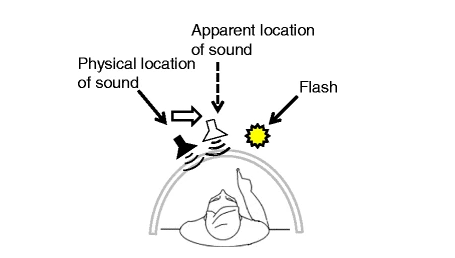
\includegraphics[width=0.55\textwidth]{04_antecedentes/figures/ventrilocuo.png}
    \caption{
        Ventriloquia espacial: la ubicación aparente de un sonido objetivo auditivo puede ser desplazada por la percepción de un estímulo visual (un destello).
    }
    \label{fig:patterns/ventrilocuo}
\end{figure}

% =============================================================================
% SECCIÓN 4: MODELOS BIOLÓGICAMENTE INSPIRADOS
% =============================================================================

\section{Modelos biológicamente inspirados}
\label{sec:modelos_biologicos}

La búsqueda de modelos computacionales que capturen los mecanismos neuronales de la cognición ha dado lugar a diversas aproximaciones, que varían en su nivel de abstracción y realismo biológico. En esta sección, vamos a revisar los principios fundamentales que guían el desarrollo de modelos biológicamente inspirados, con especial énfasis en aquellos que buscan implementar funciones computacionales mediante dinámicas neurológicamente plausibles.

\subsection{El paradigma de la ingeniería neuronal}
\label{subsec:ingenieria_neuronal}

El libro seminal \textit{Neural Engineering: Computation, Representation, and Dynamics in Neurobiological Systems} de \citet{eliasmith2003neural}, establece un marco sistemático para construir modelos que conectan la representación neuronal con la computación. Este paradigma, conocido como \textbf{ingeniería neuronal}, propone tres principios fundamentales:

\textbf{Principio 1: Representación.} Establece que las poblaciones de neuronas representan información mediante patrones de actividad distribuidos. Formalmente, si $\mathbf{x}$ es una variable que el sistema nervioso necesita representar, cada neurona $i$ en una población contribuye con una actividad:

\begin{equation}
a_i = G_i[\alpha_i \mathbf{e}_i \cdot \mathbf{x} + J_i^{bias}]
\label{eq:neural_encoding}
\end{equation}

donde $G_i[\cdot]$ es la función de transferencia de la neurona (típicamente un modelo LIF), $\alpha_i$ es un factor de ganancia, $\mathbf{e}_i$ es el ``vector de codificación'' preferido de la neurona, y $J_i^{bias}$ es una corriente de fondo \citep{eliasmith2003neural}. Este principio puede extenderse para representar no solo valores puntuales sino distribuciones de probabilidad completas.

\textbf{Principio 2: Transformación.} Especifica cómo las conexiones sinápticas entre poblaciones neuronales pueden implementar transformaciones matemáticas de las variables representadas. Dado que queremos computar una función, los pesos sinápticos óptimos pueden derivarse mediante métodos de optimización \citep{eliasmith2003neural}.

\textbf{Principio 3: Dinámica.} Describe cómo las propiedades temporales de las redes recurrentes permiten implementar sistemas dinámicos. La dinámica de una representación neuronal puede describirse mediante:

\begin{equation}
\frac{d\mathbf{x}}{dt} = f(\mathbf{x}, \mathbf{u})
\label{eq:neural_dynamics}
\end{equation}

donde $\mathbf{u}$ representa entradas externas y $f$ es la función que controla la evolución del sistema \citep{eliasmith2003neural}. Este principio es particularmente relevante cuando las dinámicas temporales, como transitorios y oscilaciones, no son meros epifenómenos sino que cumplen roles funcionales específicos en el procesamiento de información.

Estos principios proporcionan una metodología rigurosa para pasar de especificaciones funcionales a implementaciones neuronales. Sin embargo, enfoques más recientes han demostrado que es posible invertir esta lógica: partir de restricciones biológicas conocidas sobre la arquitectura de circuitos corticales, como la separación de poblaciones excitatorias e inhibitorias, funciones de transferencia supralineales, y ruido de proceso, y optimizar los parámetros para lograr una función computacional deseada, permitiendo que las dinámicas específicas emerjan como consecuencia de la optimización \citep{echeveste2020cortical}.

Independientemente del enfoque adoptado, una decisión fundamental es el nivel de detalle con que se modela la actividad neuronal. Los principios presentados pueden implementarse tanto con modelos de tasa como con modelos que capturan explícitamente los potenciales de acción individuales, cada uno con sus propias ventajas y limitaciones.

\subsection{Ruido y variabilidad neuronal}
\label{subsec:ruido_neuronal}

Una característica ubicua de la actividad neuronal es su \textbf{variabilidad}. Incluso bajo estimulación constante, las neuronas muestran fluctuaciones considerables en sus tiempos de disparo de trial a trial. Esta variabilidad, lejos de ser simplemente ``ruido'' que debe ignorarse, puede tener importantes funciones computacionales \citep{gerstner2002spiking}.

Las fuentes de variabilidad neuronal incluyen:

\begin{itemize}
    \item \textbf{Ruido de canal}: fluctuaciones estocásticas en la apertura y cierre de canales iónicos
    \item \textbf{Ruido sináptico}: variabilidad en la liberación de vesículas y en la respuesta postsináptica
    \item \textbf{Ruido de red}: actividad de fondo de otras neuronas en el circuito
\end{itemize}

En modelos computacionales, el ruido se incorpora típicamente como un término estocástico aditivo en las ecuaciones dinámicas. Un aspecto crítico es si este ruido es dependiente o independiente del estímulo. Como veremos en la Sección~\ref{sec:modelo_echeveste}, el modelo de Echeveste et al. incorpora específicamente \textbf{ruido de proceso independiente del estímulo}, una restricción biológica que resulta fundamental para las propiedades emergentes del circuito.

Crucialmente, la variabilidad neuronal puede tener un rol funcional en la inferencia probabilística. La hipótesis del \textbf{muestreo neuronal} propone que el cerebro representa distribuciones de probabilidad mediante muestras estocásticas de la actividad neuronal \citep{echeveste2020cortical}. En este marco, la variabilidad trial-a-trial no es ruido a eliminar sino una característica funcional que permite explorar el espacio de posibles interpretaciones de los estímulos sensoriales.

\subsection{Redes excitatorias-inhibitorias}
\label{subsec:redes_ei}

Partiendo de las bases del ya mencionado principio de Dale, al modelar los circuitos corticales con poblaciones separadas de neuronas excitatorias (E) e inhibitorias (I) también nos permite estudiar dinámicas que emergen de su interacción. En el régimen de \textbf{balance excitación-inhibición}, las corrientes excitatorias e inhibitorias a cada neurona se cancelan aproximadamente en promedio, manteniendo el potencial de membrana medio por debajo del umbral de disparo. En este régimen, los potenciales de acción ocurren solo cuando fluctuaciones en la entrada son suficientemente fuertes para alcanzar el umbral, generando patrones de disparo irregulares con alta variabilidad \citep{dayan2005theoretical}.

El \textbf{estado balanceado} tiene propiedades computacionalmente interesantes: genera actividad irregular similar a la observada en corteza, permite respuestas rápidas a cambios en la entrada, y puede implementar dinámicas de muestreo para inferencia probabilística \citep{echeveste2020cortical}. Estas propiedades hacen que las redes E-I balanceadas sean un punto fuerte para modelos de procesamiento cortical.

\medskip

Los principios y restricciones biológicas presentados en esta sección definen el espacio de arquitecturas biológicamente plausibles. Sin embargo, especificar la arquitectura no determina los valores de los parámetros (pesos sinápticos, constantes de tiempo) que permiten a la red realizar una función computacional específica. Para encontrar estos parámetros, los enfoques modernos recurren a técnicas desarrolladas en el campo del aprendizaje automático, que revisaremos en la siguiente sección.

% =============================================================================
% SECCIÓN 5: MACHINE LEARNING APLICADO A LA NEUROCIENCIA
% =============================================================================

\section{Machine learning aplicado a la neurociencia}
\label{sec:machine_learning}

El aprendizaje automático (\textit{machine learning}) es el campo de estudio en el cual un programa de computadora aprende de una experiencia $E$ respecto a una clase de tareas $T$ y una medida de rendimiento $P$, si su rendimiento en las tareas de $T$, medida por $P$, mejora con la experiencia $E$ \citep{mitchell1997machine}. Esta disciplina y la neurociencia han mantenido una relación simbiótica desde sus orígenes: por un lado, el cerebro ha inspirado muchos de los algoritmos de aprendizaje más exitosos, y por otro, las técnicas de machine learning proporcionan herramientas poderosas para analizar datos neuronales y desarrollar modelos computacionales del cerebro \citep{heaton2018ian}. En esta sección, revisamos los conceptos fundamentales de machine learning relevantes para el modelado neurocientífico.

\subsection{Paradigmas de aprendizaje}
\label{subsec:paradigmas_aprendizaje}

El aprendizaje automático puede clasificarse en tres paradigmas principales según la naturaleza de la señal de entrenamiento disponible \citep{bishop2006pattern, murphy2012machine}.

El \textbf{aprendizaje supervisado} opera cuando se dispone de pares entrada-salida etiquetados $\{(\mathbf{x}_i, \mathbf{y}_i)\}_{i=1}^N$. El objetivo es aprender una función $f$ que mapee entradas a salidas correctamente, típicamente minimizando una función de pérdida:

\begin{equation}
\mathcal{L} = \sum_{i=1}^N L(f(\mathbf{x}_i; \boldsymbol{\theta}), \mathbf{y}_i)
\label{eq:supervised_loss}
\end{equation}

donde $\boldsymbol{\theta}$ son los parámetros del modelo y $L$ mide la discrepancia entre predicciones y etiquetas. En el contexto neurocientífico, el aprendizaje supervisado se utiliza para entrenar redes neuronales que reproduzcan aspectos específicos de la actividad cortical o del comportamiento.

El \textbf{aprendizaje no supervisado} busca descubrir estructura en datos sin etiquetas. Esto incluye tareas como el agrupamiento (\textit{clustering}), la reducción de dimensionalidad, y la estimación de densidad. El \acrfull{PCA} es un ejemplo clásico, utilizado frecuentemente para identificar patrones de covariación en poblaciones neuronales \citep{bishop2006pattern}.

El \textbf{aprendizaje por refuerzo} considera un agente que interactúa con un ambiente y recibe señales de recompensa, aprendiendo una política que maximice la recompensa acumulada a largo plazo \citep{bishop2006pattern}.

En el contexto del presente trabajo, el paradigma relevante es el aprendizaje supervisado, aunque con una particularidad importante: en lugar de entrenar una red para producir una salida puntual correcta, el objetivo es que la \textit{distribución} de respuestas de la red coincida con una distribución objetivo. Esto requiere definir funciones de pérdida que comparen estadísticas de las respuestas (como media y covarianza) con los valores objetivo derivados de un modelo generativo. Este enfoque, desarrollado por \cite{echeveste2020cortical}, será detallado en la Sección~\ref{sec:modelo_echeveste}.

\subsection{Redes neuronales artificiales}
\label{subsec:redes_artificiales}

Las \acrfull{ANN} son modelos computacionales inspirados en la estructura del cerebro, compuestos por unidades de procesamiento interconectadas organizadas en capas \citep{heaton2018ian}. Aunque difieren significativamente de las redes biológicas en muchos detalles, capturan principios importantes de procesamiento distribuido y aprendizaje mediante ajuste de conexiones.

El \acrfull{MLP} es la arquitectura más básica. Cada capa $l$ computa:

\begin{equation}
\mathbf{h}^{(l)} = \sigma(\mathbf{W}^{(l)}\mathbf{h}^{(l-1)} + \mathbf{b}^{(l)})
\label{eq:mlp_layer}
\end{equation}

donde $\mathbf{h}^{(l)}$ son las activaciones de la capa $l$, $\mathbf{W}^{(l)}$ es la matriz de pesos, $\mathbf{b}^{(l)}$ es el vector de sesgos, y $\sigma(\cdot)$ es una función de activación no lineal \citep{heaton2018ian}.

Un avance fundamental para el entrenamiento de estas redes fue el algoritmo de \textbf{retropropagación} (\textit{backpropagation}), popularizado por \citet{rumelhart1986learning}. Este algoritmo permite ajustar los pesos de todas las capas simultáneamente, propagando los gradientes del error desde la salida hacia la entrada mediante la regla de la cadena:

\begin{equation}
\frac{\partial \mathcal{L}}{\partial \mathbf{W}^{(l)}} = \frac{\partial \mathcal{L}}{\partial \mathbf{h}^{(l)}} \frac{\partial \mathbf{h}^{(l)}}{\partial \mathbf{W}^{(l)}}
\label{eq:backprop}
\end{equation}

La importancia de este algoritmo para el campo fue reconocida con el Premio Turing 2018, otorgado a Geoffrey Hinton, Yoshua Bengio y Yann LeCun por sus contribuciones al aprendizaje profundo, y más recientemente con el Premio Nobel de Física 2024 a Hinton y John Hopfield por los fundamentos del aprendizaje automático con redes neuronales artificiales \citep{hinton2024nobel}. En el contexto del presente trabajo, la retropropagación a través del tiempo (\textit{backpropagation through time}) constituye la base para optimizar los parámetros de redes recurrentes como la de \citet{echeveste2020cortical}, donde se combina con optimizadores modernos como ADAM y L-BFGS-B.

\subsection{Arquitecturas profundas y convolucionales}
\label{subsec:arquitecturas_profundas}

El \textbf{aprendizaje profundo} (\textit{deep learning}) se refiere al entrenamiento de redes neuronales con múltiples capas ocultas. La profundidad permite aprender representaciones jerárquicas donde las capas inferiores extraen características simples y las superiores combinan estas en representaciones más abstractas \citep{heaton2018ian}.

Las \acrfull{CNN} son particularmente relevantes para el procesamiento visual. Inspiradas en la organización jerárquica del sistema visual, las CNNs aplican filtros convolucionales que son equivariantes a traslaciones:

\begin{equation}
(h * w)[i,j] = \sum_m \sum_n h[m,n] \cdot w[i-m, j-n]
\label{eq:convolution}
\end{equation}

Notablemente, CNNs entrenadas para clasificación de imágenes desarrollan representaciones en sus capas ocultas que correlacionan fuertemente con la actividad neuronal a lo largo de la jerarquía visual, desde V1 hasta corteza inferotemporal \citep{yamins2014performance}.

\begin{figure}[H]
    \centering
    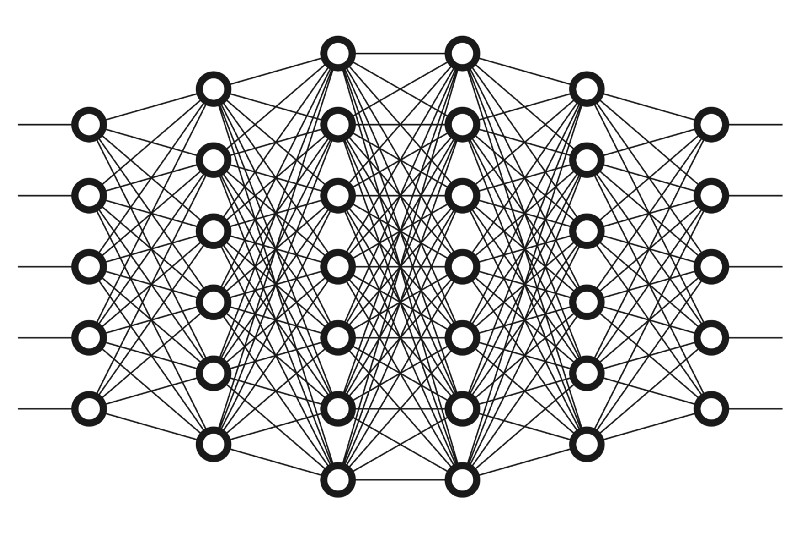
\includegraphics[width=0.55\textwidth]{04_antecedentes/figures/deep-learning.jpg}
    \caption{
        Representación de una red neuronal profunda. Se ilustra la organización en múltiples capas ocultas que permite la extracción jerárquica de características, desde rasgos simples a representaciones abstractas.
    }
    \label{fig:patterns/deep-learning}
\end{figure}

\subsection{Redes recurrentes}
\label{subsec:redes_tipo_recurrentes}

Como se discutió en la Sección~\ref{subsec:redes_recurrentes}, los circuitos corticales se caracterizan por conexiones recurrentes abundantes que permiten generar dinámicas temporales complejas. Las \acrfull{RNN} constituyen el análogo computacional de estos circuitos biológicos, extendiendo las redes feedforward al incluir conexiones que forman ciclos, permitiendo que la actividad pasada influya en el procesamiento presente \citep{heaton2018ian}. La dinámica de una RNN simple está dada por:

\begin{equation}
\mathbf{h}_t = \sigma(\mathbf{W}_{hh}\mathbf{h}_{t-1} + \mathbf{W}_{xh}\mathbf{x}_t + \mathbf{b})
\label{eq:rnn}
\end{equation}

donde $\mathbf{h}_t$ es el estado oculto en el tiempo $t$ y $\mathbf{x}_t$ es la entrada.

Arquitecturas como \acrfull{LSTM} y \acrfull{GRU} incorporan mecanismos de compuerta que permiten mantener información relevante a lo largo de secuencias largas \citep{heaton2018ian}.

En el contexto de este trabajo, las RNNs con restricciones biológicas dadas por poblaciones E-I separadas, funciones de activación plausibles y ruido de proceso, proporcionan un marco para estudiar cómo las dinámicas corticales pueden implementar funciones computacionales como la inferencia probabilística.

\begin{figure}[H]
\begin{minipage}{0.45\linewidth}
    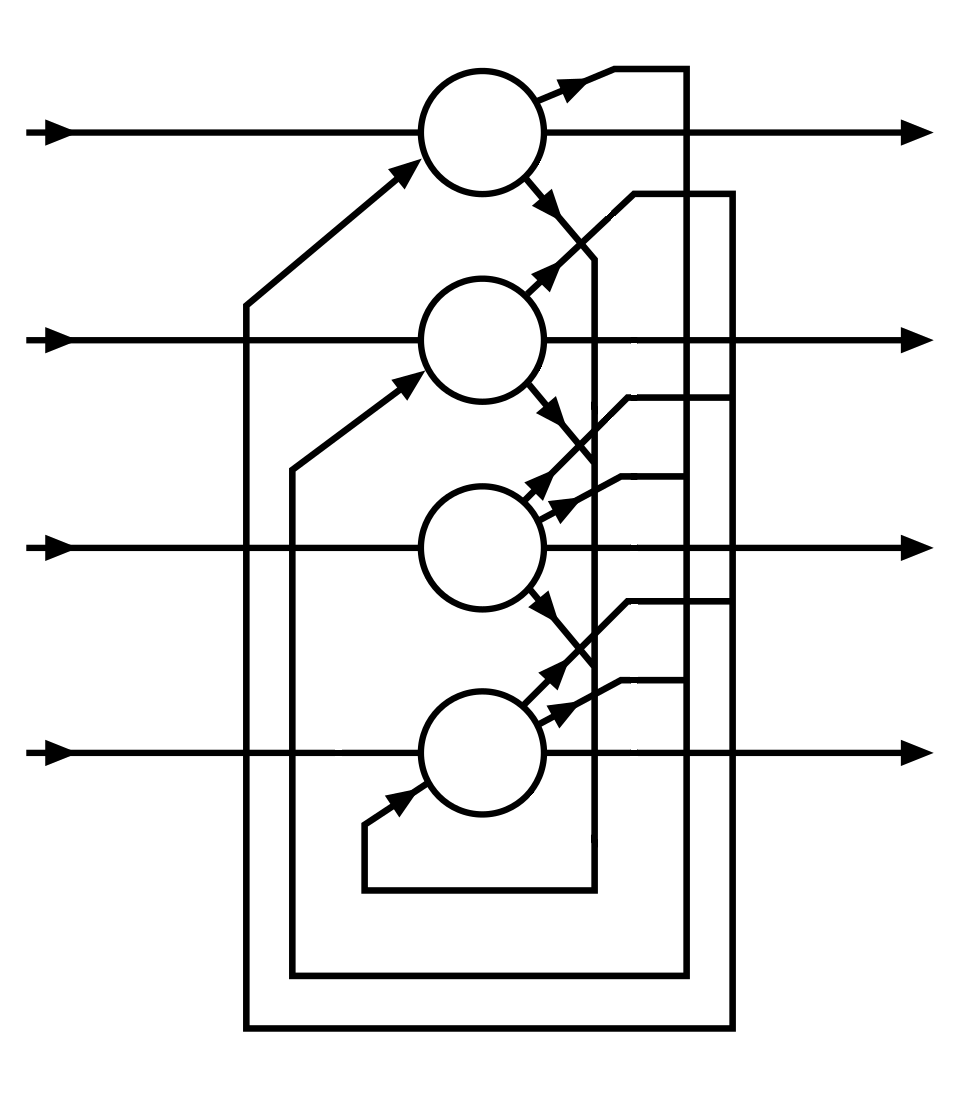
\includegraphics[width=\linewidth]{04_antecedentes/figures/rnn.png}
\end{minipage}\hfill
\begin{minipage}{0.5\linewidth}
    \caption{
        Red neuronal recurrente totalmente conectada con 4 neuronas.
    }
    \label{fig:rnn}
\end{minipage}
\end{figure}

\subsection{Estadística bayesiana y aprendizaje}
\label{subsec:bayesiana_aprendizaje}

El marco \textbf{bayesiano} proporciona una interpretación probabilística del aprendizaje donde los parámetros del modelo son tratados como variables aleatorias con distribuciones de probabilidad \citep{bishop2006pattern}. Dada una verosimilitud $P(\mathcal{D}|\boldsymbol{\theta})$ para los datos y un prior $P(\boldsymbol{\theta})$ sobre los parámetros, el teorema de Bayes proporciona la distribución posterior:

\begin{equation}
P(\boldsymbol{\theta}|\mathcal{D}) = \frac{P(\mathcal{D}|\boldsymbol{\theta})P(\boldsymbol{\theta})}{P(\mathcal{D})}
\label{eq:bayes_learning}
\end{equation}

Esta perspectiva es particularmente relevante para la neurociencia computacional. 
Diversos autores han propuesto que el cerebro opera según principios bayesianos, 
manteniendo y actualizando distribuciones de probabilidad sobre estados del mundo 
\citep{dayan2005theoretical, eliasmith2003neural}.

La \textbf{inferencia aproximada} es necesaria cuando la distribución posterior 
no puede calcularse analíticamente. Métodos como Markov Chain Monte Carlo (MCMC) 
y la inferencia variacional proporcionan aproximaciones tractables 
\citep{heaton2018ian}. Como veremos, estos métodos tienen análogos propuestos 
en dinámicas neuronales.

\subsection{Redes neuronales para inferencia probabilística}
\label{subsec:redes_inferencia}

Un aspecto fundamental para este trabajo es comprender cómo redes neuronales pueden implementar inferencia probabilística. La hipótesis del \textbf{muestreo neuronal} propone que las fluctuaciones en la actividad neuronal representan muestras de 
distribuciones de probabilidad, de modo que la actividad promediada en el tiempo corresponde a esperanzas bajo distribuciones posteriores \citep{echeveste2020cortical}.

Formalmente, si un circuito neuronal implementa muestreo de una distribución $P(\mathbf{x}|\mathbf{s})$ donde $\mathbf{s}$ es un estímulo, entonces la actividad instantánea $\mathbf{x}(t)$ representa una muestra, y:

\begin{equation}
\langle \mathbf{x}(t) \rangle_t \approx \mathbb{E}_{P(\mathbf{x}|\mathbf{s})}[\mathbf{x}]
\label{eq:neural_sampling}
\end{equation}

Esta perspectiva tiene implicaciones profundas para interpretar la variabilidad neuronal, sugiriendo que no es simplemente ruido sino que codifica incertidumbre sobre el estado del mundo.

Recientemente, se ha demostrado que redes neuronales recurrentes con restricciones biológicas pueden ser entrenadas para implementar muestreo de distribuciones posteriores complejas, mostrando simultáneamente propiedades dinámicas similares a las observadas en corteza \citep{echeveste2020cortical}. Este resultado establece un puente crucial entre la función computacional (inferencia probabilística) y los mecanismos neuronales (dinámicas corticales), y constituye un antecedente directo del presente trabajo.

% =============================================================================
% SECCIÓN 6: MODELOS Y HERRAMIENTAS PARA EL PRESENTE TRABAJO
% =============================================================================

\section{Antecedentes directos}
\label{subsec:antecedentes_directos}

Los fundamentos presentados en este capítulo, desde los mecanismos biológicos de la señalización neuronal hasta las técnicas de aprendizaje automático para optimizar redes recurrentes, proporcionan el marco conceptual y metodológico para abordar el problema central de este trabajo. En esta sección final presentamos brevemente los antecedentes específicos que, desarrollados en detalle en sus respectivos capítulos, constituyen la motivación y el punto de partida de nuestra contribución.

Entre los desarrollos que buscan implementar los principios de inferencia probabilística en arquitecturas biológicamente plausibles, dos modelos resultan particularmente relevantes para este trabajo.

El modelo de \citet{cuppini2017biologically} aborda la integración audiovisual y el efecto ventrílocuo mediante una arquitectura de tres capas que reproduce exitosamente fenómenos experimentales como el juicio de unidad. Sin embargo, al utilizar modelos de tasa deterministas, no captura las dinámicas corticales realistas observadas experimentalmente. 

En contraste, el modelo de \citet{echeveste2020cortical} demuestra que redes neuronales con restricciones biológicas pueden implementar inferencia probabilística mediante muestreo, exhibiendo propiedades emergentes como oscilaciones gamma y transitorios inhibitorios. Sin embargo, está limitado al procesamiento unimodal. Los detalles de ambos modelos están desarrollados en el Capítulo~\ref{chapter:modelos_estudiados}.

Más allá de sus diferencias conceptuales, ambos modelos comparten una limitación práctica ya que han sido implementados de manera independiente, en distintos lenguajes y con estructuras incompatibles, dificultando su comparación o integración. Para abordar este tipo de fragmentación en el campo, \citet{paredes2025scikit} desarrollaron Scikit-NeuroMSI, un framework de código abierto en Python que proporciona infraestructura común para la implementación, comparación y validación de modelos de integración multisensorial. Presentando todas sus características técnicas en el Capítulo~\ref{chapter:scikit_neuromsi}.

% \subsection{Objetivo y contribución del presente trabajo}
% \label{subsec:objetivo_contribucion}

% La revisión presentada revela una brecha significativa: los modelos de integración multisensorial como el de Cuppini capturan la arquitectura funcional pero carecen de dinámicas corticales realistas, mientras que modelos como el de Echeveste exhiben dinámicas biológicamente plausibles pero están limitados al procesamiento unimodal. Además, cada modelo ha sido implementado independientemente, dificultando cualquier intento de integración.

% La visión a largo plazo que motiva este trabajo es el desarrollo de modelos que combinen la arquitectura multimodal del modelo de Cuppini con las dinámicas corticales del modelo de Echeveste. Sin embargo, alcanzar esta visión requiere primero sentar bases técnicas sólidas. El presente trabajo representa el primer paso en esta dirección mediante la implementación del modelo de Echeveste dentro del framework Scikit-NeuroMSI.

% Esta implementación incluye la arquitectura de red con poblaciones excitatorias e inhibitorias, el modelo generativo GSM con cálculo de momentos objetivo, y el procedimiento de entrenamiento para muestreo. La validación verificará que el modelo reproduce las propiedades reportadas originalmente: convergencia de momentos, variabilidad modulada por contraste, y presencia de dinámicas temporales características.

% Junto con el modelo, el trabajo desarrolla bases para las herramientas de análisis necesarias para estudiar modelos con dinámicas temporales relevantes. Estas herramientas permitirán visualizar la evolución de los potenciales de membrana, calcular espectros de potencia para identificar oscilaciones, y comparar estadísticas de las respuestas con los valores objetivo. Aunque desarrolladas para el modelo de Echeveste, estas herramientas pueden ser modificadas y quedarán disponibles para cualquier modelo futuro que requiera análisis de dinámicas temporales.

% Es importante delimitar lo que este trabajo no aborda: la fusión con el modelo de Cuppini y la implementación de inferencia causal multisensorial quedan como direcciones futuras. El presente trabajo se enfoca en establecer las bases técnicas que harán posibles estas extensiones, reconociendo que una implementación correcta del modelo de Echeveste es condición necesaria para cualquier desarrollo posterior hacia el procesamiento multisensorial con dinámicas corticales realistas.